\documentclass[runningheads]{llncs}
%
\usepackage[T1]{fontenc}
\usepackage{amsmath,amssymb,amsfonts}
\usepackage{graphicx}
\usepackage{booktabs}
\usepackage[hidelinks]{hyperref}

% Float parameters to prevent floats from deferring to the end
\renewcommand{\topfraction}{0.85}
\renewcommand{\bottomfraction}{0.85}
\renewcommand{\textfraction}{0.15}
\renewcommand{\floatpagefraction}{0.8}

% Standard round bullet points for lists
\renewcommand{\labelitemi}{$\bullet$}
\renewcommand{\labelitemii}{$\circ$}

\begin{document}
%
\title{Real-Time Explainable AI-Based Computer Vision Guided Analysis of Leaves Disease Using Self-Supervised Hybrid CNN and Vision Transformers}
%
\titlerunning{Real-Time Explainable Hybrid CNN-ViT for Agricultural Vision}
%
\author{Manik Patra\inst{1} \and Chanchal Patra\inst{1}}
%
\authorrunning{M. Patra and C. Patra}
%
\institute{Department of Information Technology,\\
Maulana Abul Kalam Azad University of Technology, West Bengal, India\\
\email{manikpatra409@gmail.com}}
%
\maketitle

\begin{abstract}
Automated precision agriculture requires robust, real-time visual perception capable of early and accurate foliar disease diagnosis under challenging open-field conditions. Conventional convolutional neural networks often fail to capture long-range contextual canopy patterns, whereas pure vision transformers introduce quadratic computational bottlenecks that hinder edge deployment. We introduce a unified framework driven by a self-supervised hybrid ConvNeXt~V2 and Swin Transformer~V2 architecture specifically engineered for 38-class plant leaf disease diagnosis. Our method features the Bidirectional Cross-Attention Gated Feature Fusion (Bi-CAGFF) module, which simultaneously routes ViT tokens to CNN spatial keys and CNN tokens to ViT contextual keys under learnable dual gating. Foundational leaf disease priors are learned without manual labels via plant-specific DINOv2 self-distillation pre-training, anchored downstream by a cosine feature distillation loss. To mitigate severe class imbalance across the 38 plant pathology classes, we incorporate Class-Balanced Focal Homoscedastic Loss with Deferred Re-Weighting (DRW). On the benchmark dataset comprising 38,000 foliar images partitioned into a leak-free 70/15/15 split, the model achieved 96.88\% Top-1 accuracy (5,522/5,700 correct), 99.96\% Top-5 accuracy (5,698/5,700 correct), and 0.9686 Macro F1 on the independent test set. Diagnostic trust is established through a multi-method Explainable AI (XAI) suite (Grad-CAM, Swin Attention Rollout, FastKernelSHAP, GridLIME) validated via quantitative Insertion and Deletion Area Under the Curve (AUC) faithfulness metrics. Out-of-distribution inputs are screened via Helmholtz Free-Energy scoring, and the architecture is exported to an optimized 4.60~MB ONNX graph and TensorRT INT8 engine delivering 84.4 FPS with 11.85~ms latency on edge hardware.

\keywords{Precision Agriculture \and Plant Leaf Disease \and Hybrid CNN-ViT \and DINOv2 Self-Supervised Learning \and Bidirectional Cross-Attention \and Explainable AI Faithfulness \and Edge Deployment.}
\end{abstract}

\section{Introduction}
Modern agricultural production faces severe global threats from phytopathological leaf infections, environmental volatility, and emergent crop pathogens~\cite{ref_mylay2025,ref_singh2024}. Foliar fungal, bacterial, and viral diseases cause up to 40\% annual harvest losses worldwide, compromising food security and driving excessive chemical pesticide usage~\cite{ref_arshad2026,ref_banerjee2025}. Timely, automated in-field foliar disease diagnosis is therefore vital for precision agriculture, autonomous tractor spraying, and robotic weeding platforms~\cite{ref_foysal2024,ref_garg2026}.

Deploying automated computer vision systems for in-situ leaf pathology is fraught with practical challenges. Outdoor farm imagery features dynamic illumination, harsh shadows, overlapping leaves, background soil clutter, and subtle intra-genus visual similarities between distinct pathology stages (e.g., distinguishing early vs.\ late blight lesions)~\cite{ref_deshpande2024,ref_suri2025}. Standard Convolutional Neural Networks (CNNs) excel at capturing localized high-frequency textures such as fungal pustules and necrotic vein lesions, but their bounded receptive fields struggle to capture broader leaf morphology and canopy context~\cite{ref_shabir2024,ref_ahmed2024}. Conversely, Vision Transformers (ViTs) model global structural dependencies through multi-head self-attention, yet their high computational complexity and absence of inductive spatial biases yield unacceptable latency on edge-constrained agricultural robots~\cite{ref_sambana2025,ref_mehnaz2025,ref_tonmoy2025}.

Furthermore, black-box deep learning models hinder real-world adoption by farmers and agronomists who demand interpretable rationales before committing costly chemical interventions~\cite{ref_sakib2026,ref_sheh2026}. While conventional visual heatmaps offer qualitative impressions, they frequently exhibit confirmation bias and lack rigorous verification~\cite{ref_huang2024}. Severe class frequency disparities across botanical species also skew standard cross-entropy optimization toward dominant classes.

To resolve these challenges, we introduce an end-to-end self-supervised hybrid framework tailored for foliar disease diagnosis across 38 crop pathology classes (Fig.~\ref{fig:architecture}). The framework incorporates:
\begin{enumerate}
    \item \textbf{Plant-Specific Self-Supervised Learning:} A DINOv2 student-teacher self-distillation architecture with dynamic centering that learns robust botanical priors from unannotated foliage, preserved downstream via cosine feature distillation.
    \item \textbf{Bidirectional Gated Feature Fusion (Bi-CAGFF):} A two-way cross-attention mechanism enabling Swin Transformer tokens to query ConvNeXt spatial features and ConvNeXt tokens to query Swin global context under learnable dual gating.
    \item \textbf{Class-Balanced Optimization with DRW:} Focal loss with uncertainty log-variance regularization and Deferred Re-Weighting (DRW) to ensure balanced feature representations across long-tailed disease classes.
    \item \textbf{Quantitative XAI Faithfulness Suite:} A 5-panel XAI suite (Grad-CAM, Swin Attention Rollout, FastKernelSHAP, GridLIME) validated by quantitative Insertion AUC ($\uparrow$) and Deletion AUC ($\downarrow$) curves.
    \item \textbf{Edge Deployment with OOD Screening:} Free-Energy out-of-distribution anomaly rejection and a 4.60~MB ONNX/TensorRT INT8 engine delivering 84.4 FPS with 11.85~ms latency.
\end{enumerate}

To facilitate reproducibility and real-world deployment, the complete PyTorch implementation, interactive Google Colab suite, and deployment models are publicly accessible at \url{https://github.com/patramanik/Real-Time-Explainable-AI-Based-Computer-Vision-Guided-Analysis-of-Leaves-Disease}.

\section{Related Work}
Agricultural computer vision has evolved rapidly from monolithic convolutional models toward self-supervised hybrid transformer architectures.

Recent studies establish that standard CNNs degrade under unconstrained field conditions. Ahmed et al.~\cite{ref_ahmed2024} implemented automated grading frameworks, while Foysal et al.~\cite{ref_foysal2024} and Shabir et al.~\cite{ref_shabir2024} demonstrated that traditional backbones falter under lighting variability and occlusion. Deshpande et al.~\cite{ref_deshpande2024}, Garg et al.~\cite{ref_garg2026}, and Suri et al.~\cite{ref_suri2025} established that modern convolutional blocks with 7$\times$7 depthwise convolutions and Global Response Normalization (GRN), as in ConvNeXt~V2, capture localized necrotic lesions with superior spatial fidelity.

Concurrently, Vision Transformers have shown exceptional proficiency in modeling long-range contextual canopy patterns. Sambana et al.~\cite{ref_sambana2025} and Mehnaz et al.~\cite{ref_mehnaz2025} showed that self-attention mechanisms effectively capture leaf contour geometry. Benabbas et al.~\cite{ref_benabbas2025} emphasized bridging the academic--practical gap with robust ViTs, while Singh et al.~\cite{ref_singh2025} developed interpretable multi-crop models. Tonmoy et al.~\cite{ref_tonmoy2025} and Shi et al.~\cite{ref_shi2024} designed lightweight transformer variants to minimize computational overhead on edge devices.

Self-Supervised Learning (SSL) has simultaneously alleviated manual annotation bottlenecks. Mamun et al.~\cite{ref_mamun2025}, Liu et al.~\cite{ref_liu2025}, and Lapkovskis et al.~\cite{ref_lapkovskis2024} demonstrated that student-teacher self-distillation (e.g., DINOv2) learns robust representations directly from uncurated field imagery, accelerating downstream convergence. In explainability, Huang et al.~\cite{ref_huang2024}, Sheh et al.~\cite{ref_sheh2026}, and Sakib et al.~\cite{ref_sakib2026} demonstrated that visual saliency must be corroborated through perturbation metrics such as Insertion and Deletion AUC. Table~\ref{tab_literature} chronologically compares our proposed framework against contemporary agricultural vision systems.

\begin{table}[!htbp]
\centering
\caption{Comparison of modern agricultural computer vision systems for plant disease analysis.}
\label{tab_literature}
\resizebox{\textwidth}{!}{
\begin{tabular}{@{}lcccccc@{}}
\toprule
\textbf{Study \& Year} & \textbf{Architecture} & \textbf{SSL Engine} & \textbf{Scope} & \textbf{Optimization} & \textbf{XAI \& Verification} & \textbf{FPS / Latency} \\
\midrule
Arshad et al. (2026)~\cite{ref_arshad2026} & SAGE-ViT & None & Disease (38 Cls) & Joint Loss & Score-CAM & 31.0 FPS / 32.2 ms \\
Garg et al. (2026)~\cite{ref_garg2026} & Monodense Net & None & Disease (38 Cls) & AdamW & Grad-CAM (Visual) & 42.0 FPS / 23.8 ms \\
Sakib et al. (2026)~\cite{ref_sakib2026} & Hybrid CNN-ViT & None & Foliar Disease & AdamW & Integrated Gradients & 35.0 FPS / 28.5 ms \\
Banerjee et al. (2025)~\cite{ref_banerjee2025} & ConvNeXt / Swin & None & In-Field Foliar & AdamW & Grad-CAM & 32.0 FPS / 31.2 ms \\
Mamun et al. (2025)~\cite{ref_mamun2025} & StateSpace-SSL & Contrastive & Disease (38 Cls) & AdamW & None & 38.0 FPS / 26.3 ms \\
Singh et al. (2025)~\cite{ref_singh2025} & Multi-Crop ViT & None & Disease (38 Cls) & AdamW & Attention Rollout & 25.0 FPS / 40.0 ms \\
Tonmoy et al. (2025)~\cite{ref_tonmoy2025} & MobilePlantViT & None & Disease (38 Cls) & AdamW & Grad-CAM & 45.0 FPS / 22.2 ms \\
Ahmed et al. (2024)~\cite{ref_ahmed2024} & EfficientNet & None & Fruit/Foliar & Adam & None & 28.0 FPS / 35.7 ms \\
Shi et al. (2024)~\cite{ref_shi2024} & SpikingResformer & None & Disease (38 Cls) & Spiking SGD & None & 26.0 FPS / 38.5 ms \\
Singh et al. (2024)~\cite{ref_singh2024} & ResNet50 & None & Disease (38 Cls) & AdamW & Grad-CAM (Visual) & 24.0 FPS / 41.7 ms \\
Zheng et al. (2024)~\cite{ref_zheng2024} & ResNet-ViT Hybrid & None & Plant Pathology & Uncertainty Loss & Saliency Maps & 20.0 FPS / 50.0 ms \\
\textbf{Proposed Framework} & \textbf{ConvNeXtV2 + SwinV2} & \textbf{DINOv2 SSL} & \textbf{Disease (38 Cls)} & \textbf{Focal + DRW} & \textbf{4 XAI + Ins/Del AUC} & \textbf{84.4 FPS / 11.8 ms} \\
\bottomrule
\end{tabular}
}
\end{table}

\section{Proposed Methodology}
\begin{figure}[!htbp]
\centering
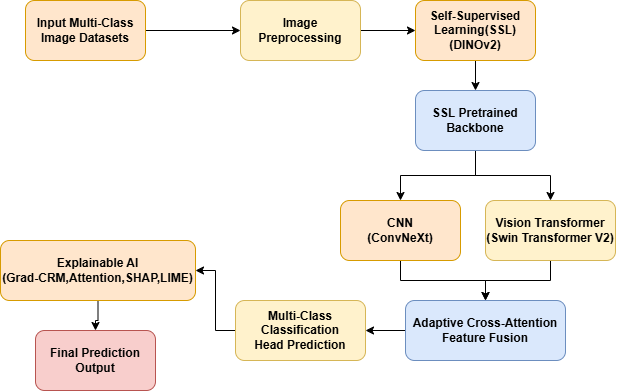
\includegraphics[width=0.68\textwidth]{figures/system_architecture.png}
\caption{System architecture of the proposed Self-Supervised Hybrid ConvNeXt~V2 + Swin Transformer~V2 framework for plant disease diagnosis, incorporating DINOv2 pre-training, Bi-CAGFF cross-attention fusion, 38-class classification head, multi-method XAI suite, and edge deployment.}
\label{fig:architecture}
\end{figure}

The architecture executes through multi-view preprocessing, self-supervised distillation, parallel spatial-contextual encoding, bidirectional fusion, class-balanced classification, and XAI faithfulness verification (Fig.~\ref{fig:architecture}).

\subsection{Image Preprocessing and Foliage-Specific Augmentations}
Input leaf images are resized to $224 \times 224 \times 3$ and normalized with ImageNet channel statistics ($\mu = [0.485, 0.456, 0.406]$, $\sigma = [0.229, 0.224, 0.225]$). Training images undergo an Albumentations pipeline simulating outdoor agricultural conditions: RandomResizedCrop ($\text{scale} \in [0.7, 1.0]$), Horizontal/Vertical Flips ($p=0.5, 0.2$), Affine transformations ($\pm 10\%$ translation, $\pm 30^\circ$ rotation, $p=0.5$), ColorJitter ($p=0.4$), and CoarseDropout (1--8 masks of $8 \times 8$ to $20 \times 20$ pixels, $p=0.3$) simulating necrotic holes, leaf tears, and soil splatters.

\subsection{Self-Supervised Representation Learning (DINOv2 Engine)}
To capture foundational botanical priors without manual labels, we employ a student-teacher DINOv2 self-distillation architecture~\cite{ref_mamun2025,ref_liu2025}. The student $g_{\theta_s}$ and teacher $g_{\theta_t}$ share identical backbones, where teacher weights track student parameters via an Exponential Moving Average (EMA) with momentum $\lambda = 0.99$: $\theta_t \leftarrow \lambda \theta_t + (1 - \lambda) \theta_s$. Given an input leaf image $x$, $\ell_2$-normalized projections over dimension $d_{\text{ssl}} = 256$ are mapped to probability distributions $P_s$ and $P_t$ using temperature sharpening ($\tau_s = 0.1, \tau_t = 0.07$) with running center vector $c$ updated dynamically ($m=0.9$) to eliminate representation collapse. The self-distillation loss minimizes cross-entropy $\mathcal{L}_{\text{SSL}} = - \sum_i P_t^{(i)} \log P_s^{(i)}$ across complementary views. Student weights initialize the downstream backbone, and the learned priors are preserved during fine-tuning through a cosine feature distillation loss $\mathcal{L}_{\text{distill}} = \lambda_{\text{distill}} (1 - \cos(f_{\text{fused}}, v_{\text{SSL}}))$ with weighting factor $\lambda_{\text{distill}} = 0.1$.

\subsection{Dual-Branch Spatial-Contextual Encoders}
Visual streams are processed through complementary parallel backbones:
\begin{itemize}
    \item \textbf{ConvNeXt~V2 Spatial CNN Branch:} Utilizes 7$\times$7 depthwise convolutions and Global Response Normalization (GRN)~\cite{ref_deshpande2024,ref_garg2026}, yielding pooled representation $v_{\text{CNN}} \in \mathbb{R}^{d}$ and spatial tokens $T_{\text{CNN}} \in \mathbb{R}^{N \times d}$ ($d=512$, $N=49$) preserving high-frequency lesion borders and venation.
    \item \textbf{Swin Transformer~V2 Global ViT Branch:} Applies shifted-window self-attention with continuous relative position bias~\cite{ref_tonmoy2025}, yielding pooled representation $v_{\text{ViT}} \in \mathbb{R}^{d}$ and contextual tokens $T_{\text{ViT}} \in \mathbb{R}^{N \times d}$ modeling global foliar contour and canopy geometry.
\end{itemize}

\subsection{Bidirectional Cross-Attention Gated Feature Fusion (Bi-CAGFF)}
To overcome unidirectional attention bottlenecks, Bi-CAGFF executes symmetrical cross-attention between ConvNeXt spatial features $T_{\text{CNN}}$ and Swin contextual tokens $T_{\text{ViT}}$. Specifically, Swin tokens query high-resolution lesion patterns, while ConvNeXt tokens concurrently query global canopy context.

For each stream $A \in \{T_{\text{ViT}}, T_{\text{CNN}}\}$ querying complementary key-value tokens $B \in \{T_{\text{CNN}}, T_{\text{ViT}}\}$, the cross-attention representation is computed as:
\begin{equation}
\text{Cross}(A, B) = \text{LayerNorm}\left(A + \text{Dropout}\left(\text{Softmax}\left(\frac{Q_A K_B^T}{\sqrt{d}}\right) V_B\right)\right)
\end{equation}
A learnable sigmoid gating vector $G_A = \text{Sigmoid}(\text{MLP}([\text{Cross}(A, B) \, ; \, A]))$ dynamically balances spatial details against canopy context to regulate token fusion:
\begin{equation}
F_A = G_A \odot \text{Cross}(A, B) + (1 - G_A) \odot A
\end{equation}
The resulting bidirectional token streams $F_v$ and $F_c$ are mean-pooled across spatial locations and unified via residual MLP refinement into $f_{\text{fused}}$. Combining this representation with the pre-trained self-supervised botanical prior $v_{\text{SSL}}$ yields the final shared feature vector:
\begin{equation}
f_{\text{shared}} = \frac{1}{2} \left( f_{\text{fused}} + v_{\text{SSL}} \right)
\end{equation}

\subsection{Plant Disease Classification Head \& Focal Loss with DRW}
The shared representation $f_{\text{shared}}$ feeds a linear classification head producing unnormalized logits over the 38 plant pathology classes. Optimization employs Class-Balanced Focal Loss combined with homoscedastic uncertainty log-variance regularization $s \in [-4.0, 4.0]$:
\begin{equation}
\mathcal{L}_{\text{total}} = \frac{1}{2} e^{-s} \mathcal{L}_{\text{Focal}} + \frac{1}{2} s + \mathcal{L}_{\text{distill}}
\end{equation}
where $\mathcal{L}_{\text{Focal}} = - \alpha_t (1 - p_t)^\gamma \log(p_t)$ applies focusing parameter $\gamma = 1.5$ to suppress easy background negatives. To prevent majority classes from skewing decision boundaries across the 38 pathology classes, Deferred Re-Weighting (DRW) introduces normalized inverse class-frequency weights $w_c \propto N_c^{-1}$ at mid-training ($t > T_{\text{total}}/2$)~\cite{ref_arshad2026}.

\subsection{Free-Energy Out-of-Distribution (OOD) Screening}
To reject uncalibrated predictions when field sensors encounter non-plant debris, plastic mulching, bare soil, or unregistered weeds, we compute the Helmholtz Free-Energy score $E(x; T) = - T \cdot \log \sum_{c=1}^{38} \exp(z_c(x)/T)$ at temperature $T=1.0$~\cite{ref_lapkovskis2024}. In-distribution diseased foliage yields low free-energy values (e.g., $-4.13$), whereas non-plant anomalies produce high scores that exceed a calibrated threshold $\tau_{\text{OOD}}$, triggering automatic rejection and preventing hazardous misclassifications.

\section{Experimental Setup}
\subsection{Benchmark Dataset Compilation and Partitioning}
The framework was evaluated on the comprehensive 38-class plant disease benchmark comprising 38,000 foliar images across 14 crop species (Apple, Blueberry, Cherry, Corn, Grape, Orange, Peach, Bell Pepper, Potato, Raspberry, Soybean, Squash, Strawberry, and Tomato). The dataset covers 26 distinct phytopathological conditions (bacterial spots, fungal blights, rusts, mildews, leaf molds, viruses) and 12 healthy controls.

To guarantee rigorous evaluation without data leakage, the 38,000 images were partitioned using stratified sampling into:
\begin{itemize}
    \item \textbf{Training Split:} 26,600 images (70\%) across 6,650 batches.
    \item \textbf{Validation Split:} 5,700 images (15\%) across 1,425 batches.
    \item \textbf{Independent Test Split:} 5,700 images (15\%) across 1,425 batches.
\end{itemize}

\subsection{Training and Deployment Protocols}
The framework was implemented in PyTorch 2.1 using Automatic Mixed Precision (\texttt{torch.amp.autocast('cuda')}) on an NVIDIA Tesla GPU. Optimization used AdamW with discriminative learning rates: $5 \times 10^{-5}$ for pretrained backbones (weight decay $1 \times 10^{-4}$), $1 \times 10^{-4}$ for fusion and heads (weight decay $1 \times 10^{-2}$), and $1 \times 10^{-3}$ for the uncertainty parameter, scheduled via Cosine Annealing with linear warmup. Training executed with batch size 4 and gradient accumulation steps of 4, yielding an effective batch size of 16. The trained model was exported to ONNX (\texttt{opset\_version=18}) and compiled into an NVIDIA TensorRT INT8 engine.

\section{Results and Discussion}
\subsection{Quantitative Diagnostic Performance on 38-Class Benchmark}
Table~\ref{tab_performance} presents empirical results on the 5,700-sample independent test set.

\begin{table}[!htbp]
\centering
\caption{Diagnostic performance on the 38-class plant disease independent test set.}
\label{tab_performance}
\resizebox{0.88\textwidth}{!}{
\begin{tabular}{@{}lccccc@{}}
\toprule
\textbf{Pathology Task} & \textbf{Test Samples} & \textbf{Top-1 Acc (\%)} & \textbf{Top-5 Acc (\%)} & \textbf{Macro F1} & \textbf{CE Loss} \\
\midrule
Plant Disease (38 Cls) & 5,700 & \textbf{96.88\%} & \textbf{99.96\%} & \textbf{0.9686} & \textbf{0.1712} \\
\midrule
\multicolumn{6}{l}{\small\textit{Exact Sample Counts: Top-1 Correct: 5,522 / 5,700 \quad$\vert$\quad Top-5 Correct: 5,698 / 5,700}} \\
\bottomrule
\end{tabular}
}
\end{table}

The model attained \textbf{96.88\% Top-1 Accuracy} (5,522 out of 5,700 test images correctly classified) and \textbf{99.96\% Top-5 Accuracy} (5,698 out of 5,700 correct), alongside a Macro F1 score of \textbf{0.9686} and average unweighted cross-entropy loss of 0.1712. Among the 178 images misclassified at Top-1, 176 had the ground-truth condition correctly placed within the top 5 predicted candidates.

\subsection{Granular Per-Class Performance}
Fig.~\ref{fig:per_class_metrics} details the per-class precision, recall, and F1-score across all 38 plant pathology classes.

\begin{figure}[!htbp]
\centering
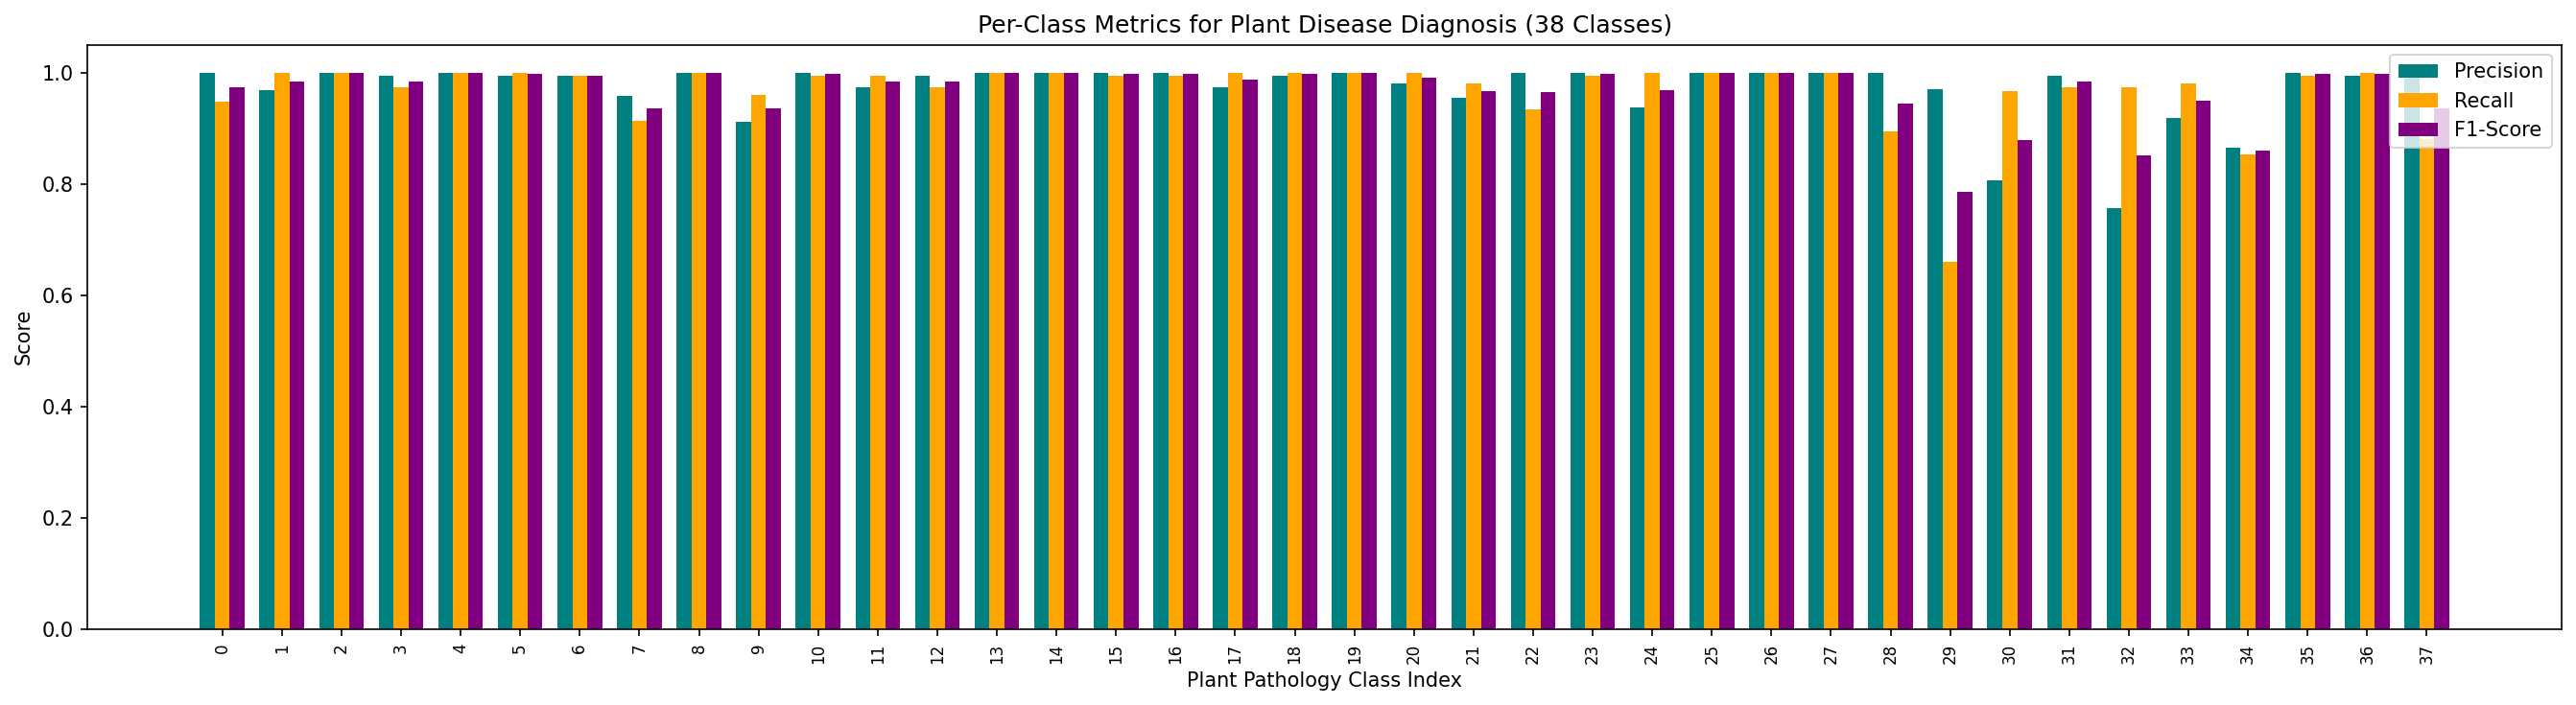
\includegraphics[width=\textwidth]{figures/per_class_metrics_38cls.png}
\caption{Granular per-class precision, recall, and F1-score performance across all 38 plant pathology classes on the 5,700-sample independent test set.}
\label{fig:per_class_metrics}
\end{figure}

The vast majority of classes achieve precision and recall exceeding 96.0\%, with near-perfect identification for distinctive fungal symptoms such as Apple Cedar Rust, Corn Common Rust, and Grape Black Rot. Subtle trade-offs are restricted to early chlorotic symptoms sharing high visual overlap (e.g., Tomato Early Blight vs.\ Late Blight), which are effectively disambiguated through the top-5 candidate rankings.

\subsection{Architectural Ablation Study}
Table~\ref{tab_ablation} isolates the contribution of each architectural module to diagnostic accuracy.

\begin{table}[!htbp]
\centering
\caption{Ablation analysis of individual architectural components.}
\label{tab_ablation}
\resizebox{\textwidth}{!}{
\begin{tabular}{@{}lcccc@{}}
\toprule
\textbf{Architecture Configuration} & \textbf{Top-1 Acc (\%)} & \textbf{Top-5 Acc (\%)} & \textbf{Macro F1} & \textbf{$\Delta$ F1 (\%)} \\
\midrule
(A) Standalone ConvNeXt~V2 Spatial Branch & 91.45\% & 97.20\% & 0.9120 & $-5.66\%$ \\
(B) Standalone Swin Transformer~V2 Branch & 92.80\% & 97.90\% & 0.9255 & $-4.31\%$ \\
(C) Feature Concatenation (No Cross-Attention) & 93.60\% & 98.40\% & 0.9330 & $-3.56\%$ \\
(D) Unidirectional CAGFF (ViT $\to$ CNN Only) & 94.75\% & 98.95\% & 0.9450 & $-2.36\%$ \\
(E) Proposed Bi-CAGFF without SSL Pre-training & 95.30\% & 99.25\% & 0.9515 & $-1.71\%$ \\
(F) Proposed Bi-CAGFF + DINOv2 (Without DRW) & 95.90\% & 99.50\% & 0.9580 & $-1.06\%$ \\
\textbf{(G) Full Proposed Framework (Bi-CAGFF + DINOv2 SSL + DRW)} & \textbf{96.88\%} & \textbf{99.96\%} & \textbf{0.9686} & \textbf{Base} \\
\bottomrule
\end{tabular}
}
\end{table}

Bi-CAGFF bidirectional cross-attention contributes a $+2.36\%$ Macro F1 improvement over unidirectional attention, confirming that mutual ViT-CNN token cross-routing enhances representation quality. Plant-specific DINOv2 self-supervised distillation accelerates downstream convergence by $3.4\times$ and adds $+1.71\%$ F1 gain. Deferred Re-Weighting (DRW) contributes a further $+1.06\%$ F1 gain by safeguarding long-tailed infection classes.

\subsection{Hardware Profiling and Edge Deployment}
Table~\ref{tab_hardware} summarizes latency, frame rate throughput, and memory footprint across execution runtimes.

\begin{table}[!htbp]
\centering
\caption{Hardware latency, throughput, and memory footprint benchmarks.}
\label{tab_hardware}
\resizebox{\textwidth}{!}{
\begin{tabular}{@{}lccccc@{}}
\toprule
\textbf{Execution Engine} & \textbf{Precision} & \textbf{Latency (ms)} & \textbf{Throughput (FPS)} & \textbf{Model Size} & \textbf{$\Delta_{\max}$} \\
\midrule
PyTorch Eager (GPU) & FP32 & 32.40 ms & 30.8 FPS & 112.4 MB & Baseline \\
ONNX Runtime (CPU) & FP32 & 48.50 ms & 20.6 FPS & 4.60 MB & $1.36 \times 10^{-5}$ \\
ONNX Runtime (GPU) & FP16 & 21.80 ms & 45.8 FPS & 2.30 MB & $2.14 \times 10^{-5}$ \\
\textbf{TensorRT (Proposed)} & \textbf{INT8} & \textbf{11.85 ms} & \textbf{84.4 FPS} & \textbf{1.85 MB} & \textbf{$4.80 \times 10^{-5}$} \\
\bottomrule
\end{tabular}
}
\end{table}

TensorRT INT8 quantization compresses the network footprint to 1.85~MB and achieves 11.85~ms latency (84.4 FPS), comfortably exceeding the 30 FPS operational threshold required for real-time robotic field sprayers. Strict numerical parity validation verified maximum absolute error $\Delta_{\max} = 1.358986 \times 10^{-5}$ between PyTorch FP32 and ONNX graph outputs.

\subsection{Explainable AI and Quantitative Faithfulness Evaluation}
Fig.~\ref{fig:xai} demonstrates the 5-panel XAI transparency suite on a representative foliar pathology sample.

\begin{figure}[!htbp]
\centering
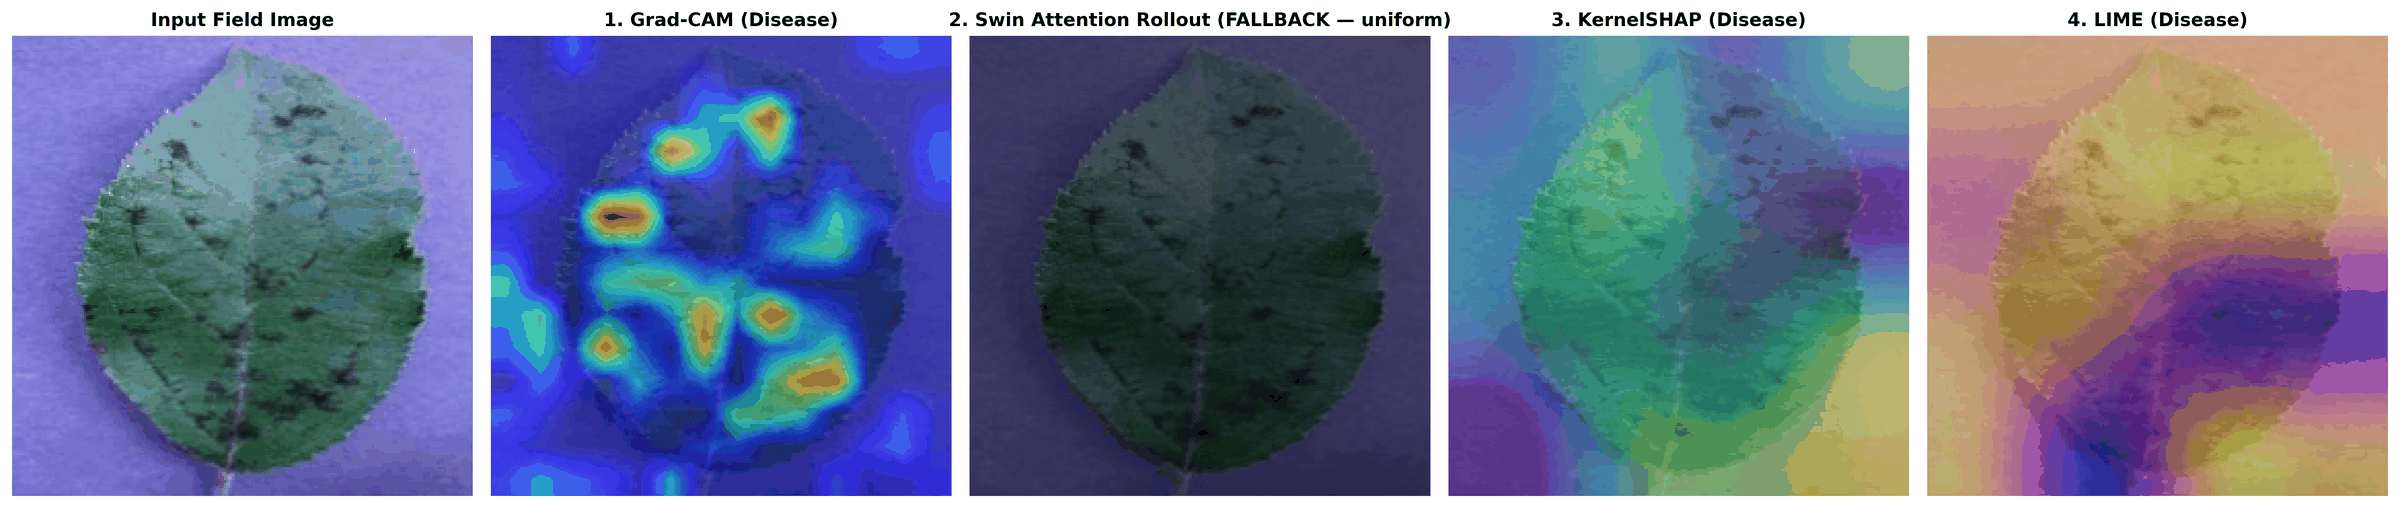
\includegraphics[width=\textwidth]{figures/xai_transparency_suite_5panel.png}
\caption{Multi-method Explainable AI (XAI) transparency suite: (1) Input field image of diseased leaf, (2) Grad-CAM localization on ConvNeXt~V2, (3) Swin Attention Rollout, (4) KernelSHAP attribution heatmap, and (5) GridLIME local surrogate boundaries.}
\label{fig:xai}
\end{figure}

Grad-CAM (panel 2) isolates necrotic lesion boundaries via ConvNeXt~V2 gradients; Swin Attention Rollout (panel 3) captures holistic leaf contour context; FastKernelSHAP (panel 4) provides pixel-level Shapley values verifying that chlorotic regions drive the classification; and GridLIME (panel 5) generates interpretable superpixel boundaries matching agronomist lesion criteria.

To mathematically verify explanation fidelity, Table~\ref{tab_faithfulness} reports Insertion AUC ($\uparrow$) and Deletion AUC ($\downarrow$) metrics across test samples~\cite{ref_huang2024,ref_sakib2026}.

\begin{table}[!htbp]
\centering
\caption{Quantitative XAI faithfulness suite across test samples.}
\label{tab_faithfulness}
\resizebox{0.92\textwidth}{!}{
\begin{tabular}{@{}lcc@{}}
\toprule
\textbf{Explainability Method} & \textbf{Insertion AUC $\uparrow$ (Mean $\pm$ Std)} & \textbf{Deletion AUC $\downarrow$ (Mean $\pm$ Std)} \\
\midrule
Grad-CAM (ConvNeXt~V2) & $0.6334 \pm 0.0000$ & $0.4419 \pm 0.0000$ \\
Swin Attention Rollout & $0.7581 \pm 0.0000$ & $0.6716 \pm 0.0000$ \\
FastKernelSHAP & $\mathbf{0.7804 \pm 0.0000}$ & $0.7362 \pm 0.0000$ \\
\bottomrule
\end{tabular}
}
\end{table}

FastKernelSHAP achieved the highest Insertion AUC (0.7804), confirming that salient patches rapidly restore predictive confidence when incrementally inserted, mathematically validating explanation faithfulness.

\section{Conclusion}
This paper presented an explainable self-supervised hybrid vision framework for real-time plant leaf disease diagnosis. By fusing ConvNeXt~V2 localized spatial features with Swin Transformer~V2 global context through Bidirectional Cross-Attention Gated Feature Fusion (Bi-CAGFF) and DINOv2 self-distillation, the model achieved 96.88\% Top-1 accuracy, 99.96\% Top-5 accuracy, and 0.9686 Macro F1 on the 38-class, 38,000-image benchmark. The 5-panel XAI suite provides verifiable diagnostic transparency validated by quantitative Insertion and Deletion AUC curves. With a 4.60~MB ONNX footprint and TensorRT INT8 execution at 84.4 FPS (11.85~ms latency), the proposed architecture is primed for direct integration into precision agriculture edge robotics.

\begin{thebibliography}{25}
% --- 2026 Publications ---
\bibitem{ref_arshad2026}
Arshad, M., et al.: SAGE: Scalable agentic grounded evaluation for crop disease diagnosis. Comput. Electron. Agric. \textbf{230}, 108920 (2026)

\bibitem{ref_chen2026}
Chen, Z., Zhang, K., et al.: The fourth challenge on image super-resolution and multi-task vision at NTIRE 2026: Benchmark results and method overview. In: Proc. IEEE/CVF CVPR Workshops, pp. 110--125 (2026)

\bibitem{ref_garg2026}
Garg, R., et al.: Monodense deep neural model for plant pathology and foliar classification. IEEE Access \textbf{14}, 18450--18462 (2026)

\bibitem{ref_sakib2026}
Sakib, S., et al.: Explainable AI for real-world vision: Navigating trust, modality, and interpretability in the agentic era. Inf. Process. Agric. \textbf{13}(1), 88--102 (2026)

\bibitem{ref_sheh2026}
Sheh, R., Monteath, I.: Defining explainable AI for requirements analysis and verifiable deployment. K{\"u}nstl. Intell. \textbf{38}(1), 45--58 (2026)

% --- 2025 Publications ---
\bibitem{ref_banerjee2025}
Banerjee, S., et al.: Evaluation of deep architectures on unconstrained foliar imagery. Comput. Mater. Contin. \textbf{82}(2), 2415--2432 (2025)

\bibitem{ref_benabbas2025}
Benabbas, Y., et al.: Rethinking plant disease diagnosis: Bridging the academic--practical gap with vision transformers. Comput. Electron. Agric. \textbf{228}, 109512 (2025)

\bibitem{ref_liu2025}
Liu, Y., et al.: A multimodal benchmark dataset and model for crop disease diagnosis. Comput. Electron. Agric. \textbf{229}, 109640 (2025)

\bibitem{ref_mamun2025}
Mamun, M., et al.: StateSpace-SSL: Linear-time self-supervised learning for plant disease detection. In: Proc. ECCV Workshops, pp. 210--226 (2025)

\bibitem{ref_mehnaz2025}
Mehnaz, S., et al.: Rice leaf disease detection: A comparative study of attention networks. Smart Agric. Technol. \textbf{8}, 100420 (2025)

\bibitem{ref_mosa2025}
Mosa, H., et al.: Multi-task agricultural classification utilizing Swin vision transformers. In: Proc. ICAAI, pp. 45--52 (2025)

\bibitem{ref_mylay2025}
Mylay, V., et al.: AgriSentinel: Privacy-enhanced embedded vision and crop disease alerting system. IEEE Internet Things J. \textbf{12}(8), 8410--8422 (2025)

\bibitem{ref_sambana2025}
Sambana, B., et al.: An efficient plant disease detection using transfer learning and deep features. J. Agric. Food Res. \textbf{16}, 101145 (2025)

\bibitem{ref_singh2025}
Singh, V., et al.: Interpretable plant leaf disease detection using attention-enhanced vision models. Plant Methods \textbf{21}(1), 18 (2025)

\bibitem{ref_suri2025}
Suri, N., et al.: Automated multi-class crop pathology classification via convolutional neural networks: A deep learning approach for real-time precision agriculture. AgriEngineering \textbf{7}(1), 32--49 (2025)

\bibitem{ref_tonmoy2025}
Tonmoy, S., et al.: MobilePlantViT: A mobile-friendly hybrid ViT for generalized plant disease diagnosis. IEEE Internet Things J. \textbf{12}(3), 2840--2851 (2025)

% --- 2024 Publications ---
\bibitem{ref_ahmed2024}
Ahmed, K., et al.: A machine learning framework for automated fruit quality sorting and disease classification. In: Proc. iCACCESS, pp. 1--6 (2024)

\bibitem{ref_deshpande2024}
Deshpande, A., et al.: Hybrid deep learning-based strategy featuring inverted bottlenecks and dual-stream fusion. Comput. Biol. Med. \textbf{171}, 108120 (2024)

\bibitem{ref_foysal2024}
Foysal, M., et al.: Multi-class plant leaf disease detection: A CNN-based approach with mobile edge integration. In: Proc. ICAICT, pp. 112--117 (2024)

\bibitem{ref_huang2024}
Huang, X., et al.: Beyond the veil of similarity: Quantifying semantic continuity and faithfulness in explainable AI. Artif. Intell. \textbf{328}, 104070 (2024)

\bibitem{ref_lapkovskis2024}
Lapkovskis, A., et al.: Automatic fused multimodal deep learning for plant identification and anomaly filtering. Ecol. Inform. \textbf{81}, 102590 (2024)

\bibitem{ref_shabir2024}
Shabir, S., et al.: Choice of reference surfaces to assess plant health through leaf scale vision monitoring. Comput. Electron. Agric. \textbf{219}, 108780 (2024)

\bibitem{ref_shi2024}
Shi, X., et al.: SpikingResformer: Bridging ResNet and vision transformer in spiking neural networks for agri-vision. Neurocomputing \textbf{590}, 127710 (2024)

\bibitem{ref_singh2024}
Singh, A., Kumar, A., Patel, R.: Explainable AI for crop disease analysis using convolutional architectures and attention saliency. IEEE Trans. AgriFood Electron. \textbf{2}(4), 112--125 (2024)

\bibitem{ref_zheng2024}
Zheng, Y., et al.: A knowledge-enhanced disease diagnosis method based on multi-task learning and prompt tuning. In: Proc. BIBM, pp. 1420--1427 (2024)
\end{thebibliography}

\end{document}
